\documentclass{article}
\usepackage{graphicx}
\usepackage[utf8]{inputenc}
\begin{document}

\title{Git}
%\author{Author's Name}

\section*{Introduction}
\subsection*{Snapshots}
-Git speichert seine Daten nicht als Serie von Änderungen oder Unterschieden, sondern als Serie von Schnappschüssen. \\
\begin{figure}[h!]
    \centering
    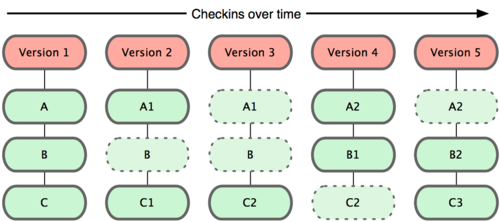
\includegraphics[width=\textwidth]{../bilder/snap.png}
    \caption{Git speichert Daten als eine Historie von Snapshots des Projektes.}
    \label{snap}
\end{figure} 
	
- Dies ist ein wichtiger Unterschied zwischen Git und praktisch allen anderen Versionskontrollsystemen, welche Veränderungen speichern.

\subsection*{Fast jede Operation ist lokal}
Die meisten Operationen in Git benötigen nur die lokalen Dateien und Ressourcen auf dem lokalen Rechner. Im Allgemeinen werden keine Informationen von einem anderen Rechner im Netzwerk benötigt. Weil man die vollständige Historie auf dem Rechner hat, werden die allermeisten Opertationen schnell ausgeführt.

\subsection*{Integrität}
Änderungen in Git werden in Checksummen umgerechnet, bevor sie gespeichert werden. Anschließend werden sie mit dieser Checksumme referenziert. Das macht es unmöglich, dass sich die Inhalte von Dateien oder Verzeichnissen ändern, ohne dass Git das mitbekommt.

Fast alle Operationen, die Du in der täglichen Arbeit mit Git verwendest, fügen Daten jeweils nur zur internen Git Datenbank hinzu. Deshalb ist es sehr schwer, das System dazu zu bewegen, irgendetwas zu tun, das nicht wieder rückgängig zu machen ist, oder dazu, Daten in irgendeiner Form zu löschen.

\subsection*{Die drei Zustände}
Git hat drei Zustände, in denen sich die Dateien befinden können: \textit{commited, modified und staged}: \\
-Commited heißt, dass die Datei sicher in der lokalen Datenbank gespeichert ist. \\
-Modified bedeutet, dass die Datei geändert wurde, aber die Änderung noch nicht commited wurde. \\
-Staged heißt, dass eine geänderte Datei in ihrem veränderten Zustand für den nächsten Commit vorbereitet ist. \\ \\
Das führt uns zu den drei Hauptbereichen eines Git-Projektes:

\begin{figure}[h!]
    \centering
    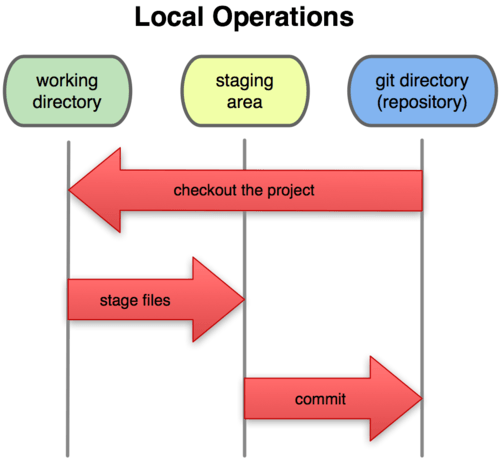
\includegraphics[width=\textwidth]{../bilder/zustand.png}
    \caption{Working Tree, Staging Area und Git-Directory (Repo)}
    \label{zustand}
\end{figure} 

Das git-directory ist der Ort, an dem Git die Metadaten und die lokale Datenbank für das Projekt speichert. Dieser Teil wird kopiert, wenn man ein anderes Repo von einem anderen Rechner klont.

Der Working tree (das Arbeitsverzeichnis) ist ein einzelner Checkout einer spezifischen Version des Projektes. Die Dateien im Working directory (= working tree) werden aus der Datenbank des git-directories geholt und auf der Festplatte so gespeichert, dass sie genutzt und bearbeitet werden können.

Die staging area ist eine Datei (normalerweise im git-directory) in der vorgemerkt wird, was in den nächsten Commit soll. \\ \\
Der basic git-worklow sieht dann wie folgt aus:\\
1. man arbeitet and Dateien im working tree\\
2. man staged individuell die Veränderungen, die Teil des nächsten Commits sein sollen, man fügt also diese Veränderungen der stagin area zu\\
3. man führt einen Commit durch: die Dateien in der staging area werden in einem snapshot dem git-directory permanent hinzugefügt

Wenn eine Datei gestaged wird, wird fuer sie eine Checksum erstellt und in der staging area gespeichert.

\section*{Git konfigurieren}

\subsection*{aliases}

\section*{Begriffe}
\subsection*{head/Head}

HEAD ist ein pointer auf den localen Branch auf dem man gerade ist

\subsection*{staging}
Die Staging-Area 



-Man pusht und pullt Commits von einem Repo in ein anderes.\\

\section*{git clone}
Dient dazu, ein vorhandenes Repo als Ziel festzulegen und einen Klon oder eine Kopie des Ziel-Repos zuerstellen.
Mit clone kopiert man ein bestehendes Repo und die Arbeitskopie ist ein vollwertiges Git-Repo mit eigenem Verlauf, eigenem Dateimanagement und einer vom ursprünglichen Repo komplett isolierten Umgebung.

Beim Klonen wird automatisch eine Remot-Verbindung namens \textit{'origin'} erstellt (Verweis auf ursprüngliches Repo).

Mit \textit{git clone} wird jede einzelne Version jeder einzelnen Datei in der Historie des Repositorys heruntergeladen

\subsection*{git clone $<$url$>$ $<$directory-name$>$}
Legt einen Ordner mit dem Namen \textit{directory-name} an, falls dieser nicht gegeben ist mit dem repo namen des zu klonenden repos. In dem neuen Ordner wird ein git-directory angelegt. Es werden alle Daten des repos runtergeladen und eine Arbeitskopie der letzen Version ausgecheckt.

\section*{git status, git add}
Ist das Maintool, um zu sehen, welche Dateien in welchem Zustand sind.
Dateien können untracked sein, was bedeutet, dass Git diese Datei nicht im vorherigen Snapshot getrackt hat. Um eine noch nicht getrackte Datei zu tracken, benutzt man \textit{git add}. Die Datei ist nun getrackt und für den nächsten Commit gestaged. Wenn eine Datei modifiziert wurde, kann die geänderte Datei ebenfalss mit \textit{git add} gestaged werden. 

\textit{git add} ist also ein Comand mit mehrere Anwendungen, es kann zB. ebenfalls dafür genutzt werden, um merge-conflict files als resolved zu markieren.

Wenn man eine Datei bearbeitet und staged und dann nochmal bearbeitet, ist die Datei bei \textit{git status} sowohl als staged, als auch als not staged gelistet. Git staged eine Datei genau so, wie sie war, als \textit{git add} ausgeführt wurde. Wenn man nun committed, wird die Version beim \textit{git add}-Befehl von der Datei in den Commit aufgenommen. Möchte man also die aktuelle Version committen, muss man die Datei erneut stagen.

\section*{git diff}

\section*{git commit}

Alles was unstaged ist, wird nicht in den nächsten Commit aufgenommen, bleibt jedoch in der aktuellen Version im working-tree vorhanden.
\textit{git commit} öffnet den Standardtexteditor mit einem text-hinweis, sowie standardmäßig dem output von \textit{git status} vor dem commit. Dazu kann man dann seine commit-message schreiben.

Jedes mal, wenn man einen Commit erstellt, nimmt man einen Snapshot vom Projekt auf zu dem man zurückkehren oder den man zum Vergleichen nutzen kann.

Wenn man in Git commitet, speichert Git ein Commit-Objekt. Dieses enthält einen Zeiger zu dem Schnappschuss mit den Objekten der staging-area, dem Autor, den Commit-Metadaten und einen Zeiger zu den direkten Eltern des Commits (Ein initialer Commit hat keine Eltern-Commits, ein normaler Commit stammt von einem Eltern-Commit ab und ein Merge-Commit, welcher aus einer Zusammenführung von zwei oder mehr Branches resultiert, besitzt ebenso viele Eltern-Commits).

\subsection*{git commit -v}
Das Selbe wie oben, aber zusätzlich zum \textit{git status} output wir noch die \textit{git diff} von den Änderungen mit im Editor angezeigt, zum besseren Überblick über Geändertes. \\\\
Alternativ dazu kann man die commitmessage auch im Terminal mit \textit{git commit -m "$<$message$>$"} direkt eingeben.

\subsection*{Die Staging Area skippen}
Fügt man -a zum \textit{git commit}-Befehl hinzu, lässt Git automatisch jede veränderte, getrackte Datei stagen und direkt commiten.

\subsection*{Dateien löschen}
Um eine Datei aus dem git-directory zu löschen, muss man sie von den tracked files entfernen (genauer aus der stagin area entfernen). \textit{git rm} macht genau das und entfernt die entsprechende Datei auch aus dem aktuellen working directory, dass man sie beim nächsten Commit nicht mehr als untracked sieht.

Wenn man die Datei einfach aus dem working-directory entfernt, dann erscheint die Datei als deleted unter \textit{Changes not staged for commit}. Wenn man nun git rm ausführt, dann wird  das entfernen gestaged und beim nächsten Commit ist die Datei dann weg und wird nicht mehr getracked. Wenn man diese Datei aber modifiziert, oder schon gestaged hat, muss man das Entfernen mit -f forcen, da versehentliches Löschen von Dateien, die noch nicht im git-directory liegen verhindert werden soll.

Manchmal möchte man vielleicht die Datei im Working Tree behalten, aber sie aus der staged-area entfernen, zB. wenn man versehentlich eine Datei gestaged hat, die noch nicht in .gitignore steht, aber eigentlich nicht committed werden soll. In diesem Fall benutzt man die \textit{--cached}-option:  \textit{git rm --cached $<$filename$>$}, um die Datei filename zu unstagen.

Man kann \textit{git rm} Dateien, Ordner und glob-Dateimuster übergeben.

\subsection*{Dateien moven (umbenennen)}
\textit{git mv README.md README} ist äquivalent zum externen Umbenennen, Removen der alten Datei und Adden der "Neuen".

\subsection*{git log}

\section*{Änderungen rückgängig machen}
Achtung: Hier kann man echt was falsch machen!

\subsection*{Den letzten Commit verbessern}
Hat man zB. einen Fehler in der commit-message gemacht, oder eine Datei aus Versehen nicht gestaged, bietet sich die commit-Option \textit{--amend} an.
Hat man sich bei der commit-message vertan, gibt führt man \textit{git commit --amend} aus und es öffnet sich der Standardtexteditor, in dem man die alte message korrigieren kann. Es bleibt der selbe Commit mit neuer message und der mit der falschen message wird durch den Neuen ersetzt.

Genau mit dem selben Command lassen sich nachträglich zu einem Commit ungestagede Dateien nachträglich in einen Commit einbauen, von dem man ebenso die message überarbeiten kann. Der neue Commit ersetzt dann den alten.

\subsection*{Eine Datei unstagen}
Um eine Datei, die man verändert hat, aber nicht committen will, aber versehentlich gestaged hat zu unstagen schlägt einem \textit{git status} den folgenden Befehl vor:
\textit{git reset HEAD $<$file$>$}. Nach dem Command ist die Datei unstaged, behält aber ihre Veränderung bei. \textit{git reset} wird später genauer erklärt.

\subsection*{Eine Modifizierung rückgängig machen}
Möchte man Änderungen an einer Datei rückgängig machen, d.h. sie auf den Stand des letzten Commits resetten, schlägt einem \textit{git status} den Befehl \textit{git checkout -- $<$file$>$} vor. Achtung, mit diesem Befehl können versehentlich gewollte Änderungen, die noch nicht im git-directory sind gelöscht werden.

Wenn man die Änderungen gerne behalten, aber die Datei jetzt noch nicht haben möchte, da man beispielsweise neue Funktionalitäten erst testen möchte, werden später stashing und branching interessant.

\section*{Mit Remotes arbeiten}
Remote Repositories sind Versionen eines Projektes, die im Internet oder einem anderen Netzwerk gehosted werden (kann auch bei einem selbst sein).

\subsection*{git remote}
Mit \textit{git remote} kann man sich anzeigen lassen, welche remoten Server man konfiguriert hat. Es werden die Namen aller Remote-Handels die angegeben wurden angezeigt. Nachdem man ein Repo gecloned hat, sollte mindestens 'origin' angegeben werden. (origin ist der default-name, den Git dem Server gibt, von dem gecloned wurde.)

\subsection*{git remote -v}
Mit der Option -v lassen sich die URLs fuers lesen und schreiben zu den Abkuerzungen angeben.

\subsection*{Remotes hinzufuegen, git remote add $<$shortname$>$ $<$url$>$}
Um ein neues remote Git-Repo unter einer Abkuerzung hinzuzufuegen, nutzt man folgenden Befehl \textit{git remote add $<$shortname$>$ $<$url$>$}. Hat man so nun zB. ein Repo eines anderen Mitarbeiters unter dem shortname \textit{pb} geadded, kann man sich die neusten Aenderungen von ihm mit \textit{git fetch pb} herunterladen.

\subsection*{git fetch $<$remote$>$}
Mit git fetch lassen sich die neuen remote-Aenderungen herunterladen, die im lokale git-directory noch nicht vorhanden sind. Und es werden lokal neue Referenzen zu den geladenen branches erstellt (remote/master, remote/branch1, etc.).

\subsection*{git pull}
Wenn der aktuelle Branch konfiguriert ist, einem remote-branch zu folgen, kann man zum downloaden und automatischen mergen \textit{git pull}-command verwenden. In diese Befehl ist \textit{fetch} mit eingebaut und es findet direkt nach dem fetchen noch ein merge in den aktuell ausgecheckten Branch statt.

Standardmaessig konfiguriert \textit{git clone} den lokalen master-branch so, dass er den remote-master branch trackt.

\subsection*{git push $<$remote$>$ $<$refspec$>$}
$<$remote$>$ ist das Zielrepo des push Vorgangs und $<$refspec$>$ setzt sich wie folgt zusammen: $<$source$>$:$<$destination$>$. $<$source$>$ ist oft der branch-name von der branch, den ich pushen will und $<$destination$>$ gibt an, welche Referenz vom remote mit dem push geupdated werden soll.

Laesst man das \textit{:destination} weg, wird der remote-branch mit dem selben Namen wie $<$source$>$ geupdated.		??????

Dieses Command funktioniert nur, wenn man ueber die noetigen Zugriffsrechte verfuegt und niemand sonst in der Zwischenzeit gepusht hat. In letzterem Fall, muessen erst die neuen Aenderungen in die lokale Version eingebaut werden.

\subsection*{Inspecting a Remote}
\subsection*{Renaming and Removing Remotes}

\section*{Tagging}



\section*{git branch}
Branching bedeutet, dass man sich von der Haupt-commit-Linie abspaltet und parallel in einem neuen Branch weiterarbeitet, ohne das Hauptprogramm zu beeinflussen.

\subsection*{Introduction}
Angenommen man hat einen Ordner mit drei Dateien und staged alle. Dann werden fuer alle drei je die Checksum generiert, welche in die staging area geadded werden. Zusaetzlich werden die Versionen der Dateien im git-directory gespeichert (sog. blob).

Wenn man dann committed, checksumt Git jedes subdirectory (jeden Unterordner) und speichert als ein Tree-Objekt im git-directory. Das Tree-Objekt enthaelt den Inhalt des Ordners und es gibt an unter welchem Namen welche blobs gespeichert sind.

Als naechstes erzeugt Git ein commit-Objekt mit den Meta-Daten (Autor, Commit-Message, etc.), mit einem Pointer zum Root-Tree, um gegebenefalls den Snapshot wieder zu erzeugen.

Das git-repo enthaelt nun 5 Objekte: ein Tree-Objekt, 3 Blobs und ein Commit-Objekt mit dem Pointer auf den root-tree.

\begin{figure}[h!]
    \centering
    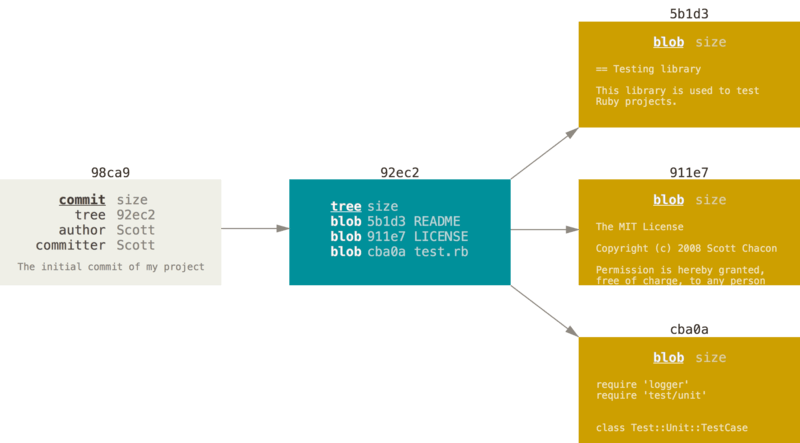
\includegraphics[width=\textwidth]{../bilder/branch1.png}
    \caption{Beispiel-Git-Directory nach dem ersten Commit}
    \label{branch1}
\end{figure} 

Die naechsten Commits werden noch pointer auf ihre Parent-commits speichern.
In der naechste Grafik ist eine Folge von Commits nach Veraenderungen dargestellt.

\begin{figure}[h!]
    \centering
    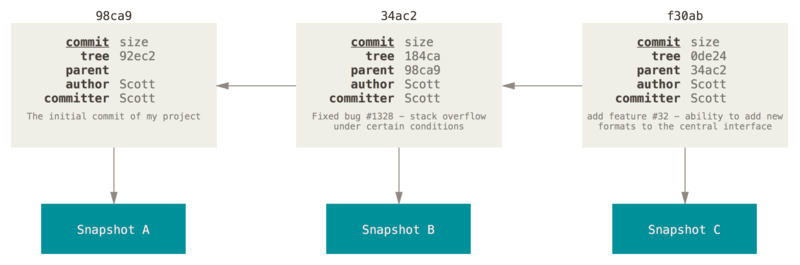
\includegraphics[width=\textwidth]{../bilder/branch2.png}
    \caption{Commits und Verknuepfung zu Eltern}
    \label{branch2}
\end{figure} 

\subsection*{Branch}
Ein Branch ist nichts anderes als ein leicher, aenderbarer Pointer, welcher auf Commits zeigen kann.

\textit{git init} erzeugt standardmaessig den branch master, welcher aber nicht anders ist als alle anderen branches.

Immer wenn man committed, wandert der branch-pointer automatisch mit zum neuen nachsten Commit.
Erstellt man nun einen neuen branch mit \textit{git branch $<$new-branch-name$>$}, wird ein neuer Pointer erstellt, welcher bei Erstellung noch auf den aktuellen Commit zeigt.

\subsection*{HEAD}
Damit Git weiss, mit welchem branch man gerade arbeitet, nutzt es einen speziellen Pointer namens HEAD, welcher immer auf den aktuellen, lokalen Branch zeigt (auf den branch auf dem man gerade arbeitet).


In der folgenden Grafik wird das noch einmal dargestellt: Es gibt zwei branches, welche beide auf den neusten Commit zeigen, sowie den pointer HEAD, welcher auf den master-branch zeigt.

\begin{figure}[h!]
    \centering
    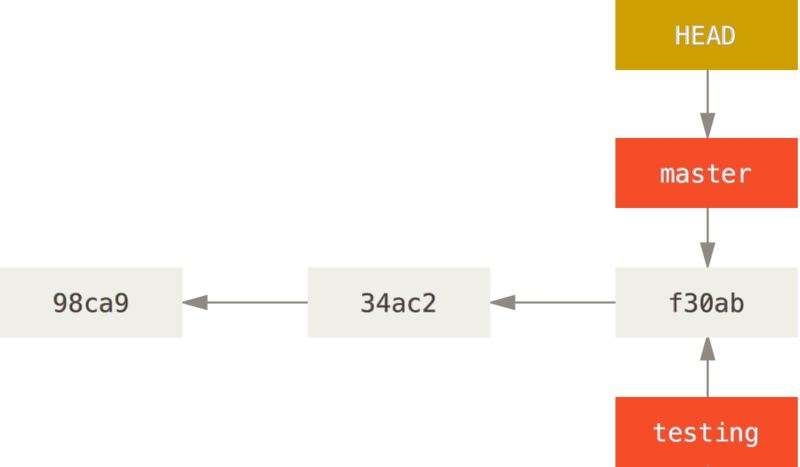
\includegraphics[width=\textwidth]{../bilder/head.png}
    \caption{HEAD und branches}
    \label{head}
\end{figure} 

\textit{git branch} erzeugt lediglich einen neuen branch, es wird nicht direkt zu diesem gewechselt.

\subsection*{git log --oneline}
Mit diesem Befehl laesst sich schnell anzeigen auf welche commits die branches zeigen und auf welchen branch HEAD zeigt.
   
\subsection*{git checkout}
Um auf einen anderen branch zu wechseln nutzt man den Befehl \textit{git checkout $<$branch$>$}. Dadurch wird HEAD auf den angegebenen branch gesetzt. Beim checkout wird also der HEAD verschoben und wandert immer mit, wenn in dem aktuellen branch ein neuer commit gemacht wird.

Um einen neuen branch zu erstellen und direkt zu ihm zu switchen, nutzt man das Command \textit{git checkout -b $<$newbranchname$>$}

Angenommen man switcht auf den branch 'testing' und committed dort eine Aenderung, geht zurueck auf den master-branch, aendert dort etwas und committed erneut. Dann laesst sich das branch-setting wie folgt darstellen:

\begin{figure}[h!]
    \centering
    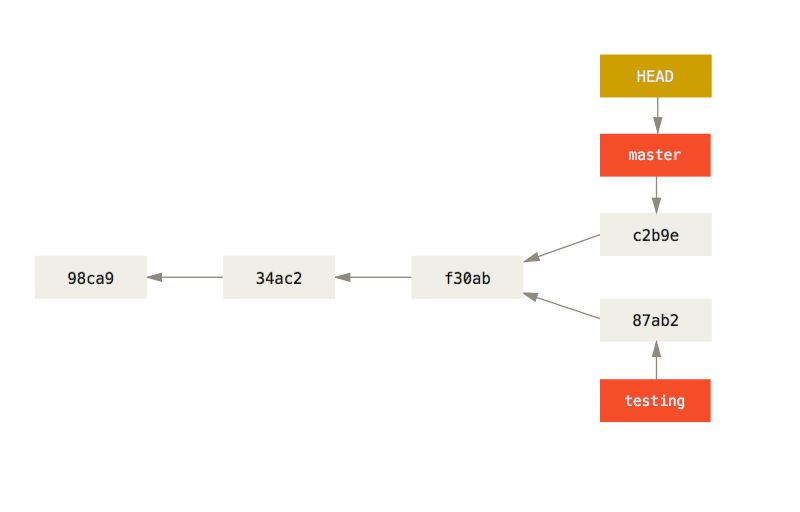
\includegraphics[width=\textwidth]{../bilder/branch3.png}
    \caption{Aufgespaltener Commit-Verlauf}
    \label{branch3}
\end{figure} 

Um zu einem anderen branch zu wechseln, muessen beim aktuellen branch alle Aenderungen, die noch nicht comitted sind, comitted werden.

\subsection*{Merging}

\subsection*{Remote branches}

Remote references sind Referezen (pointer) im remote repo (branches, tags, etc.).

\subsection*{remote-tracking branches}
Remote-tracking branches sind lokale Zeiger zu einem Zustand (commit?) des remote repositorys. Sie koennen von einem selbst nicht verschoben werden, sondern werden von Git verschoben, wenn man uebers Netzwerk mit dem remote repo kommuniziert, um immer den aktuellen state des remote repos zu repreasentieren. Man kann sie sich so vorstellen wie Lesezeichen die anzeigen, wie das remote repo das letzte Mal aussah, als man mit ihm interagiert hat.

Sie haben die Form $<$remote$>$/$<$branch$>$.\\\\
Ein Beispiel:

\begin{figure}[h!]
    \centering
    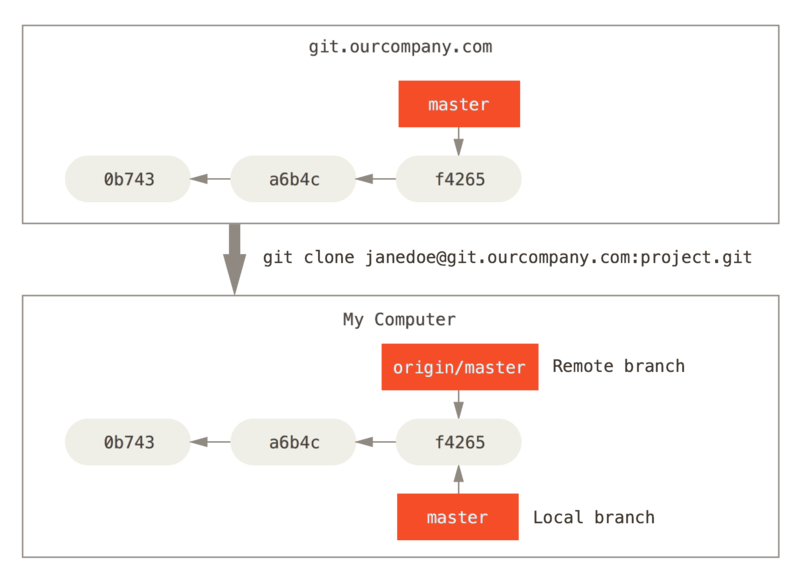
\includegraphics[width=\textwidth]{../bilder/remote-branches-1.png}
    \caption{Branch-Erzeugung beim clonen eines remote repositorys}
    \label{remoote1}
\end{figure} 

Wenn nun jemand waehrend man selbst arbeitet und committed auf das remote Aenderungen pusht und damit den remote master-branch weiterschiebt, verschiebt sich der lokale remote-tracking branch erst mit einem \textit{git fetch $<$remote$>$} Befehl entsprechend der Aenderungen, die geladen werden:

\begin{figure}[h!]
    \centering
    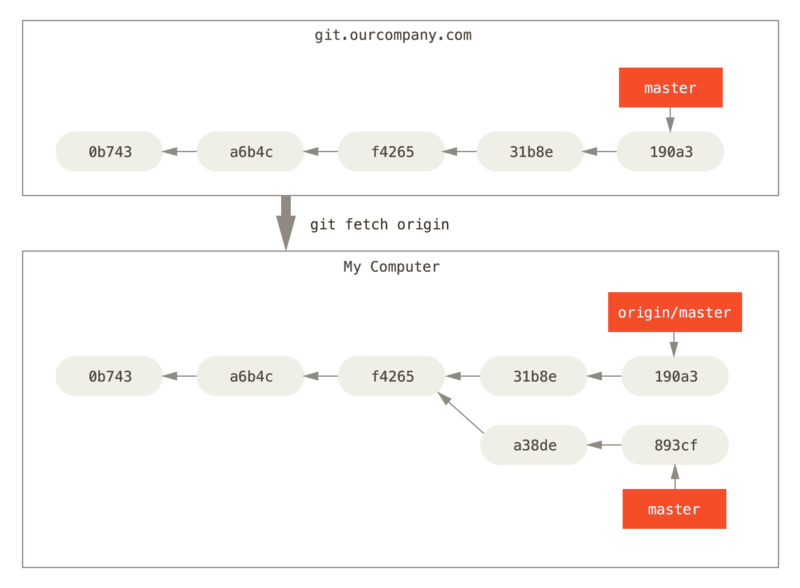
\includegraphics[width=\textwidth]{../bilder/remote-branches-3.png}
    \caption{Remote-tracking branch wird nach fetchen entprechend der remote-Aenderungen verschoben}
    \label{remoote2}
\end{figure} 

\subsection*{multiple remote servers}

\subsection*{pushing to branches}
Die lokalen branches werden nicht automatisch mit den remote branches synchronisiert. Man muss die branches, die man teilen moechte explizit pushen.

Mit dem Command \textit{git push origin serverfix} wird der current branch auf den branch serverfix des origin remotes gepusht. Git ersetzt dabei den ausdruck \textit{serverfix} mit \textit{refs/heads/serverfix:refs/heads/serverfix}, was so viel bedeutet, wie 'Nimm meinen lokalen branch serverfix und update damit den remote-branch serverfix'. Man koennte auch wie oben schon erwaehnt schreiben \textit{git push origin serverfix:serverfix}.

Es ist wichtig zu wissen, dass man, wenn man einen fetch durchfuehrt, der einen neuen remote-tracking branch mit sich bringt, nicht direkt auch einen lokalen branch zu diesem remote-tracking branch hat. Entweder merged man sich den branch mit seinem current branch zusammen (\textit{git merge origin/serverfix}), oder man erstellt sich einen neuen lokalen branch, welcher auf dem remote-tracking branch basiert (git checkout -b serverfix origin/serverfix), was einen neuen branch erzeugt, welcher dort startet, wo der remote-tracking branch startet und direkt HEAD auf diesen neuen branch setzt.

\subsection*{Tracking branches}
Tracking branches sind lokale branches, die eine direkte Verbindung zu einem remote-branch haben. Wenn man sich in einem tracking branch befindet und \textit{git pull} ausfuehrt, dann weiss Git direkt, von wo gefetch werden und was gemerged werden soll.

\end{document}